
\section{Understanding GSN Virtual Sensors}

The internal behaviour of GSN is of a content-based publish-subscribe
system, on which subscribers (virtual sensors) are subscribed (using
SQL queries) to publishers (wrappers). Content (sensor data) is
described as timestamped tuples and stored in tables in a relational
database.  GSN handles the storage and event notifications internally.

All this is implemented in GSN as follows:

\begin{enumerate}
	\item When a wrapper is loaded, a table is created and given a random name.
The table's fields are obtained from the DataField[] array defined in
the wrapper code. This table will be use to store any data coming from
the sensor and it will be automatically timestamped.
	\item When a virtual-sensor is loaded, several things happen. First, a
view\footnote{http://en.wikipedia.org/wiki/Database\_view

} is created from the wrapper table based on the SQL query specified
in the \begin{math}<\end{math}source\begin{math}>\end{math} section in
the virtual-sensor XML file\footnote{ In GSN terms, this is know as the
\textquotedblleft{}source query\textquotedblright{}.

}.  The SQL query in this section is used to
\textquotedblleft{}select\textquotedblright{} which data fields from
the wrapper table are selected for the view. This step is repeated for
any number of data sources declared in the virtual-sensor XML file.
Second, once the view is created (internally), a table is created for
the virtual-sensor, the size of this table is declared in the
virtual-sensor XML file in the
\begin{math}<\end{math}storage\begin{math}>\end{math} section, and the
name of the table is the name given to the virtual-sensor. The data
fields of this table are obtained from the
\begin{math}<\end{math}output-structure\begin{math}>\end{math} section
in the virtual-sensor XML file and they have to match with the SQL
query section \begin{math}<\end{math}stream\begin{math}>\end{math}
section\footnote{This is know as the \textquotedblleft{}virtual sensor
query\textquotedblright{}.

}.
\end{enumerate}



Note that most of this is hidden from the user, in this document we
will describe how this is implemented in GSN.



A \textbf{Virtual Sensor} (\textit{VS}) is the main component in gsn.
It receives data from one or more \begin{math}Wrapper(s)\end{math}. It
can combine their data, process and finally store it. A \textit{VS} is
defined in a single  Virtual Sensor Description file (\textit{VSD)} and
combines different pieces of software

\begin{itemize}
	\item One Virtual Sensor Processing Class (\textit{VSP})
	\item Zero or Many \begin{math}Wrapper(s)\end{math}
\end{itemize}

Depending on the actual virtual sensor used, the processed data may be
published as a data stream, displayed as a chart, sent to a database or
used in any number of ways limited only by the ingenuity of the
developer.

The GSN software includes a library of standard virtual sensors and a
framework that facilitates the development of others.  The
configuration of any specific instance of a virtual sensor is defined
in an XML document called a virtual sensor definition (VSD).

We use the multiFormatSample virtual sensor, a fairly basic instance
of a virtual sensor to demonstrate and follow the flow of data using
the Bridge Virtual Sensor.  The flow of data in this basic sensor is
depicted in the following illustration:

%\includegraphics[width=462pt]{img0.eps}
\begin{figure}%[htb]
  \centering
  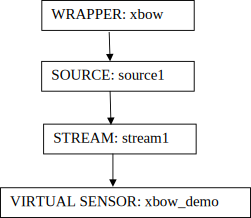
\includegraphics[width=0.4\columnwidth]{vs-dataflow}
  \caption{}
  \label{fig:tutorial-vs}
\end{figure}

\subsection{The multiFormatSample Virtual Sensor.}

We will use the MultiFormat wrapper
(src.gsn.wrappers.MultiFormatWrapper.java) since it is the simplest
wrapper to study (and modify) and the wrapper
\textquotedblleft{}simulates\textquotedblright{} a sensor which
provides temperature, light, and packet type sensor readings every
second but does not actually rely on an external data source for its
operation.

\subsection{Virtual Sensor Description File }

A \textbf{Virtual Sensor Description file} (\textit{VSD}) is an XML
file that contains the selection and the parameterization of the
\textit{VSP} and wrapper that compose a \textit{VS}.  This file also
contains the SQL statements that connect them together.

The multiFormatSample Virtual Sensor is defined by the following
virtual-sensor XML file:

\begin{xmlcode}[caption={multiFormatSample.xml}, label=listing:mfs-vs]
<virtual-sensor name="MultiFormatTemperatureHandler" priority="10">
	<processing-class>
		<class-name>gsn.vsensor.LightVirtualSensor</class-name>
		<init-params />
		<output-structure>
			<field name="light" type="double"/>
			<field name="temperature" type="double"/>
			<field name="packet_type" type="int/>
		</output-structure>
	</processing-class>
	<description>Simulates sensor readings every second.</description>
	<life-cycle pool-size="10" />
	<addressing>
		<predicate key="geographical">Sensor 114 @ EPFL</predicate>
		<predicate key="LATITUDE">46.520000</predicate>
		<predicate key="LONGITUDE">6.565000</predicate>			
	</addressing>
	<storage history-size="10"/>
	<streams>
		<stream name="input1">
			<source alias="source1" sampling-rate="1" storage-size="1">
				<address wrapper="multiformat">
					<predicate key="HOST">localhost</predicate>
					<predicate key="PORT">22001</predicate>
				</address>
				<query>SELECT light, temperature, timed FROM wrapper</query>
			</source>
 			<query>source1.light AS light_sensorFROM source1</query>
		</stream>
	</streams>
</virtual-sensor>
\end{xmlcode}


Listing  multiFormatSample.xml

\subsection{Wrapper}

A GSN Wrapper (Wrapper) is a piece of Java code that does the data
acquisition for a specific type of device..

The wrapper from which the data will be selected is defined in the
address element of the source, for example in multiFormatWrapper:

\begin{xmlcode}
				<address wrapper="multiformat">
					<predicate key="HOST">localhost</predicate>
					<predicate key="PORT">22001</predicate>
				</address>
\end{xmlcode}


The predicates included in the address element are parameters that are
particular to the wrapper used.  As the multiFormat wrapper generates
its own data the address predicates are not really required but are
included for illustration only.

In a wrapper that connects to an external data source, the predicates
contain parameters necessary to identify the instance of the wrapper to
be used.  In this case, if the wrapper connected to a real data sourse,
the parameters would define a network host address and port to connect
to the sensor.

The wrapper creates a table from the DataField[] structure:

\begin{xmlcode}[caption={DataField declaration in multiFormatWrapper.java}, label=listing:xml:data-field]
private DataField[] collection = new DataField[] { 
	new DataField("packet_type", "int", "packet type"), 
	new DataField("temperature", "double", "Presents the temperature sensor."),
	new DataField("light", "double", "Presents the light sensor.") };
\end{xmlcode}

When GSN is started, wrappers tables are given randomly generated
names, for example, the table for the MultiFormatWrapper in this
instance is given the name \_501577155. If we query that table (see),
we notice the following fields: timed, PACKET\_TYPE, TEMPERATURE,
LIGHT, and a primary key field PK. Some of the data fields are
automatically converted to upper case by GSN for clarity. These fields
correspond to the ones defined in the DataField[]array in the wrapper
code:

The timed field is automatically generated by GSN to indicate the
timestamp of the tuple. The timestamp is expressed in unix epoch time.

\begin{table*}[!htp]
	\centering
	{\normalfont\footnotesize
	\begin{tabulary}{\textwidth}{|C|C|C|C|J|}%
	\hline
		\multicolumn{5}{|c|}{\textbf{multiFormat Wrapper data table}} \\
	\hline
	\hline
		\textbf{PK} &
		\textbf{timed} &
		\textbf{PACKET\_TYPE } &
		\textbf{TEMPERATURE} &
		\textbf{LIGHT} \\
	\hline
	  386 & 1225841381231 & 1 &	NULL & 779 \\
	\hline
	  387 & 1225841382591 & 1 & NULL & 329.2 \\
	\hline
	\end{tabulary}
	}
	\caption{multiFormat Wrapper data table}
	\label{table:wrapper-table}
\end{table*}

Once the wrapper code is initialized and the wrapper table created
then when a virtual-sensor is loaded,  a view or a set of views is
created to represent the data source

\subsection{Source}

The source element of the VSD includes the wrapper declaration and an
SQL query to select the required data:

\begin{xmlcode} 	
<source alias="source1" sampling-rate="1" storage-size="1">
		<address wrapper="multiformat">
			<predicate key="HOST">localhost</predicate>
			<predicate key="PORT">22001</predicate>
		</address>
		<query>SELECT light, temperature, timed FROM wrapper</query>
	</source>
\end{xmlcode}

The attributes of the source include:

\textit{alias}\hspace{15pt}an identifier for this source

\textit{storage-size}\hspace{15pt}the window size - the number of data
items stored in the temporary table which sets the number of record
used to calculate aggregate functions such as AVG, MIN, MAX or SUM.  In
the example, no aggregate is used so the value is set at 1.  (In the
sample, two rows are present because the sample was viewed after a new
record was recieved but before the previous one was dropped.

\textit{slide}\hspace{15pt}the amount by which the sliding window
moves when generating aggregate queries.  For example, a slide value of
10 would generate a query on the arrival of each tenth record.  (slide
is not relevant to queries not using aggregate funcions such as the
present example.)

\textit{sampling-rate}\hspace{15pt}provides for load shedding when the
source generates data at a higher rate than required.  Has a value
between 0 and 1.  A value of 1 means no data is dropped, while a value
of 0.2 means only 20\% of data items will be processed and the
remainder (80\%) will be silently dropped.

The data view for source1 is named \_695753603and contains the
following data fields: light, temperature, packet type and timed (see
).

\begin{table*}[!htp]
	\centering
	{\normalfont\footnotesize
	\begin{tabulary}{\textwidth}{|C|C|C|J|}%
	\hline
		\multicolumn{4}{|c|}{\textbf{SELECT * FROM \_695753603;}} \\
	\hline
	\hline
		\textbf{light} &
		\textbf{temperature} &
		\textbf{packet\_type } &
		\textbf{timed} \\
	\hline
	  329.2 & NULL & 1 & 1225841382591\\
	\hline
	\end{tabulary}
	}
	\caption{Source data view}
	\label{table:source-view}
\end{table*}


Since views are virtual tables created by stored queries. This view
corresponds to the \textquotedblleft{}source\textquotedblright{} query
defined in the virtual-sensor XML file (). In this way, if several data
sources are declared, GSN can use views to
\textquotedblleft{}merge\textquotedblright{} data from wrapper tables,
in other words, views act as temporary tables to hold data used by
virtual-sensors.

\subsection{Stream}

A stream tells GSN what data to send to the result table created for
the virtual sensor.  The stream declaration defines the source views
from which data will be selected and the SQL query to select data to be
added to the table:

\begin{xmlcode}
<stream name="input1">
	<source alias="source1" sampling-rate="1" storage-size="1">
		<address wrapper="multiformat">
			<predicate key="HOST">localhost</predicate>
			<predicate key="PORT">22001</predicate>
		</address>
		<query>SELECT light, temperature, timed FROM wrapper</query>
	</source>
	<query>source1.light AS light_sensorFROM source1</query>
</stream>
\end{xmlcode}

The attributes of a stream include:

\textit{name}\hspace{15pt}a mandatory identifier for the stream.

\textit{rate}\hspace{15pt}The rate parameter is a performance tuning
parameter. It defines the minimum interval in milliseconds between two
calls to this virtual sensor. If there is data available for the
virtual sensor in less than this value, then the data is silently
dropped (Book of GSN p. 25).

\textit{count}\hspace{15pt}Count puts a limit on the life cycle of the
stream query in terms of number of outputs.

For instance, if the count is 100 it implies that the stream source
should become disabled after producing 100 values (stream elements).
This property is used rarely and it is planned to be 
removed from the next release. 

The stream query selects data from one or more sources and can perform
joins to combine data from multiple sources.  The result set of the
query is inserted into a table bearing the name of the virtual sensor
which becomes the output of the sensor.  The `timed' field can be
selected from one of the sources or failing that the time at the GSN
container host will be used.

\begin{table*}[!htp]
	\centering
	{\normalfont\footnotesize
	\begin{tabulary}{\textwidth}{|C|C|C|C|C|}%
	\hline
	\multicolumn{5}{|c|}{\textbf{SELECT * FROM multiformattemperaturehandler;}} \\
	\hline
	\textbf{PK} &
	\textbf{timed} &
	\textbf{LIGHT} &
	\textbf{TEMPERATURE} &
	\textbf{PACKET\_TYPE} \\
	\hline
  74552 &	1225841363432 &	 637.9 	&        NULL &	           1 \\ \hline
  74553 &	1225841364792 &	 507.3 	&        60.2 &	           2 \\ \hline
  74554 &	 1225841368402 &	  NULL &	     17.3 &	           2 \\ \hline
  74555 &	 1225841369042 &	 691.9 &       NULL &	           1 \\ \hline
  74556 &	 1225841372136 &	 380.3 &	     NULL &	           1 \\ \hline
  74557 &	 1225841375230 &	 834.5 &	     NULL &	           1 \\ \hline
  74558 &	 1225841376059 &	  NULL &	     60.1 &	           2 \\ \hline
  74559 &	 1225841378168 &	  NULL &	     75.7 &	           2 \\ \hline
  74560 &	 1225841381231 &	   779 &	     NULL &	           1 \\ \hline
  74561 &	 1225841382591 &	 329.2 &	     NULL &	           1 \\ \hline
	\end{tabulary}
	}
	\caption{multiFormat VS Output Table}
	\label{table:vs-out}
\end{table*}



\subsection{Virtual Sensor}

The root element of the VSD is labelled
\begin{math}<\end{math}virtual-sensor\begin{math}>\end{math} and
contains attributes that define the whole VS

\textit{name}\hspace{15pt}is a mandatory and arbitrary identifier for
the VS which can be used by another virtual sensor to idntify this
virtual sensor as a source using the remote or local virtual sensor
class.

\textit{priority}\hspace{15pt}is optional and must be between 0 which
is the highest priority and 20 is the lowest. The default priority is
10.

\subsubsection{Virtual Sensor Processing Class}

A \textbf{Virtual Sensor Processing class} (\textit{vsp}) is a piece
of Java code that process and stores the data upon reception from the
wrapper.

\begin{xmlcode}
	<processing-class>
		<class-name>gsn.vsensor.LightVirtualSensor</class-name>
		<init-params />
		<output-structure>
			<field name="light" type="double"/>
			<field name="temperature" type="double"/>
			<field name="packet_type" type="int/>
		</output-structure>
	</processing-class>
\end{xmlcode}
The key elements in this section are:

\textit{class-name}\hspace{15pt}specifies the name of a java class
that implements the virtual sensor processing class (VSP).
(gsn.vsensor.BridgeVirtualSensor is used in the example).  The GSN
distribution includes several VSP's and a framework in which others can
can be developed.

\textit{unique-timestamps}\hspace{15pt}allows the virtual sensor to
override the default which is to make the index to the timestamp
UNIQUE.  This would allow duplicated timestamps to be added to the
table.

\textit{init-params}\hspace{15pt}allows for the provision of
parameters to the virtual sensor class.  Parameters are specific to
individual sensor classes.

\textit{output-specification-rate} acts in a similar manner to the
rate attribute of a stream but presumably controls the the whole VS
rather than an individual stream.  In a VS with only one stream both
seem to have the same effect which is to pevent the generation of
another data row until the specified time (in milliseconds) has
elapsed.

\textit{output-structure}\hspace{15pt}provides the structure of a row
in the output data.  The name and type attributes of each field element
must match those of a data item selected in the stream query.  The text
contents of each field element can contain an optional description of
the field.

\subsubsection{Other Elements of a VSD}

Other elements of the \textit{VSD} include:

\textit{description }can contain a textual description of the sensor.

\textit{life-cycle pool-size }is a performance parameter.  It is
usually safe to keep the default value.  It defines the maximum number
of instances of this virtual sensor (with this configuration). This can
happen when the processing method of the virtual sensor takes a long
time to complete, and / or when data arrives at high speed. If all
instances are busy, then the data will be dropped.

The \textit{addressing} element contains predicates which can be used
to specify the location and other characteristics of the virtual
sensor.  The predefined keys
\textquotedblleft{}LATITUDE\textquotedblright{} and
\textquotedblleft{}LONGITUDE\textquotedblright{} can be used to locate
the sensor on the map pages of the web interface.

\textit{storage history-size} sets the number of records to be
retained in the virtual sensor table.  It does not impact the logical
processing of data streams.

\subsection{Summary}

The multiFormatSample VS is a very simple example which simply selects
data fields in the stream from a single wrapper.  The examples were
generated using release 890 of GSN and MySQL as the underlying
database.

The real power of GSN lays in its ability to use more complex SQL
queries with multiple data streams, sources and wrappers but that can
only be approached with any confidence once the basics are understood.

